% !TeX spellcheck = en_GB
\documentclass{beamer}\mode<presentation>{\usetheme{AMSBolognaFC}}
\setbeamertemplate{bibliography item}{\insertbiblabel}

\usepackage{common}

\newcommand{\labN}{12}
\newcommand{\labGroup}{https://dvcs.apice.unibo.it/pika-lab/courses/ds/ay2223}
\newcommand{\labRepo}{\labGroup/lab-\labN}

\title[L\labN{} -- Queues]{L\labN{} -- Queues}
%
\subtitle[SD]{Distributed Systems / Technologies}
%
\author[Ciatto et al.]
{Giovanni Ciatto \and Andrea Omicini \and \emph{Matteo Magnini}\\
\texttt{giovanni.ciatto@unibo.it \and andrea.omicini@unibo.it \and matteo.magnini@unibo.it}}
%
\institute[DISI, Univ. Bologna]
{Dipartimento di Informatica -- Scienza e Ingegneria (DISI)\\\textsc{Alma Mater Studiorum} -- Universit{\`a} di Bologna a Cesena}
%
\date[A.Y. 2022/2023]{Academic Year 2022/2023}

\setbeamercovered{transparent}

\AtBeginSection[]
{
\begin{frame}[c]\frametitle{Next in Line\ldots}
%    \begin{multicols}{2}
        \tableofcontents[sectionstyle=show/shaded, subsectionstyle=show/hide, subsubsectionstyle=hide/hide]
%    \end{multicols}
\end{frame}
}

\AtBeginSubsection[]
{
    \begin{frame}[c]\frametitle{Next in Line\ldots}
        %    \begin{multicols}{2}
        \tableofcontents[sectionstyle=show/shaded, subsectionstyle=show/hide, subsubsectionstyle=show/hide]
        %    \end{multicols}
    \end{frame}
}

\begin{document}

\maketitle

\begin{frame}[c]\frametitle{Outline}
    % \begin{multicols}{2}
	    \tableofcontents[sectionstyle=show/show, subsectionstyle=show/show, subsubsectionstyle=show/show]
    % \end{multicols}
\end{frame}

\section{Queues}

\begin{frame}{Overview}

    Yet another powerful abstraction for DS: \alert{queues}
    %
    \begin{columns}
        \begin{column}{.26\linewidth}
            \begin{center}
                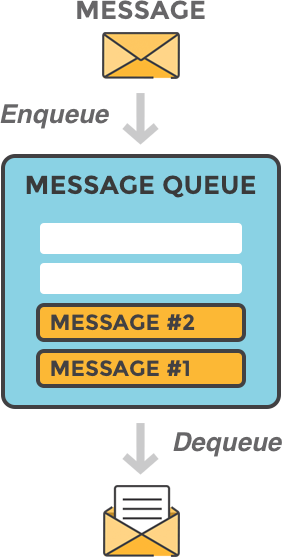
\includegraphics[width=\linewidth]{img/queue.png}
            \end{center}
        \end{column}
        \hfill
        \begin{column}{.72\linewidth}
            \begin{itemize}
                \item \alert{mono-directional}, like byte streams
                %
                \begin{itemize}
                    \item two operations: enqueue \& dequeue
                \end{itemize}

                \smallskip

                \item carrying discrete \alert{messages}, like RPC
                %
                \begin{itemize}
                    \item serialized as byte chunks
                \end{itemize}

                \smallskip

                \item commonly \alert{buffered} \& unlimited
                %
                \begin{itemize}
                    \item to support \alert{time-uncoupling}
                \end{itemize}

                \smallskip

                \item commonly, \alert{non-blocking}

%                \smallskip
%
%                \item commonly backed by ad-hoc \alert{protocols}
%                %
%                \begin{itemize}
%                    \item[eg] AMQP, MQTT, etc.
%                \end{itemize}
            \end{itemize}
        \end{column}
    \end{columns}
\end{frame}

\begin{frame}[allowframebreaks]{Producers, Consumers, Brokers}

    \begin{block}{Major roles}
        \begin{center}
            Producers $\rightarrow$ Broker $\rightarrow$ Consumers
        \end{center}
        %
        \begin{description}
            \item[producers:] pro-actively enqueuing messages into queues
            \item[consumers:] dequeuing messages from queues
            %
            \begin{itemize}
                \item either pro-actively or reactively
            \end{itemize}
            \item[brokers:] buffering queues' messages while ``in transit''
        \end{description}
    \end{block}
    %
    \begin{center}
        
\includegraphics[width=\linewidth]{img/broker.png}
    \end{center}

    \framebreak

    \begin{block}{A \textbf{broker}\ldots}
        %
        \begin{itemize}
            \item is needed to support \alert{time uncoupling}
            \item relies upon some \alert{message queueing} protocol (e.g. AMQP)
            %
            \begin{itemize}
                \item natural support for messages and acks + QoS guarantees
            \end{itemize}
            \item is an \alert{infrastructural} component
            %
            \begin{itemize}
                \item[ie] it should not appear in the abstract design of a system
            \end{itemize}
        \end{itemize}
    \end{block}

    \framebreak

    \begin{alertblock}{Notice that}
        \begin{itemize}
            \item technically, both producers and consumers are \alert{clients} w.r.t. the broker
            \item depending on your design producers and consumers may act as:
            %
            \begin{itemize}
                \item service providers or consumers
                \item or peers
            \end{itemize}
        \end{itemize}
    \end{alertblock}

\end{frame}

\section{RabbitMQ}

\begin{frame}{Overview \hfill \uurl{https://www.rabbitmq.com/}}

    \begin{itemize}
        \item Very mature MQ broker technology based on AMQP

        \vfill

        \item Supporting many programming languages and platforms
        %
        \begin{itemize}
            \item namely Python, Java, Ruby, PHP, C\#, JavaScript, Go, Elixir, Objective-C, Swift
            \item via as many \alert{client libraries}
        \end{itemize}

        \vfill

        \item The broker is written in Erlang
        %
        \begin{itemize}
            \item can be started via its Docker container: \uurl{https://hub.docker.com/_/rabbitmq}
        \end{itemize}

        \vfill

        \item Major abstractions
        %
        \begin{description}
            \item[queues] | actual buffers storing messages
            \item[exchanges] | gateways towards one or more queues
            \item[routing] | the operation of selecting which queues a message should be forwarded to
        \end{description}

    \end{itemize}
\end{frame}

\begin{frame}{Workflow}


    \begin{center}
        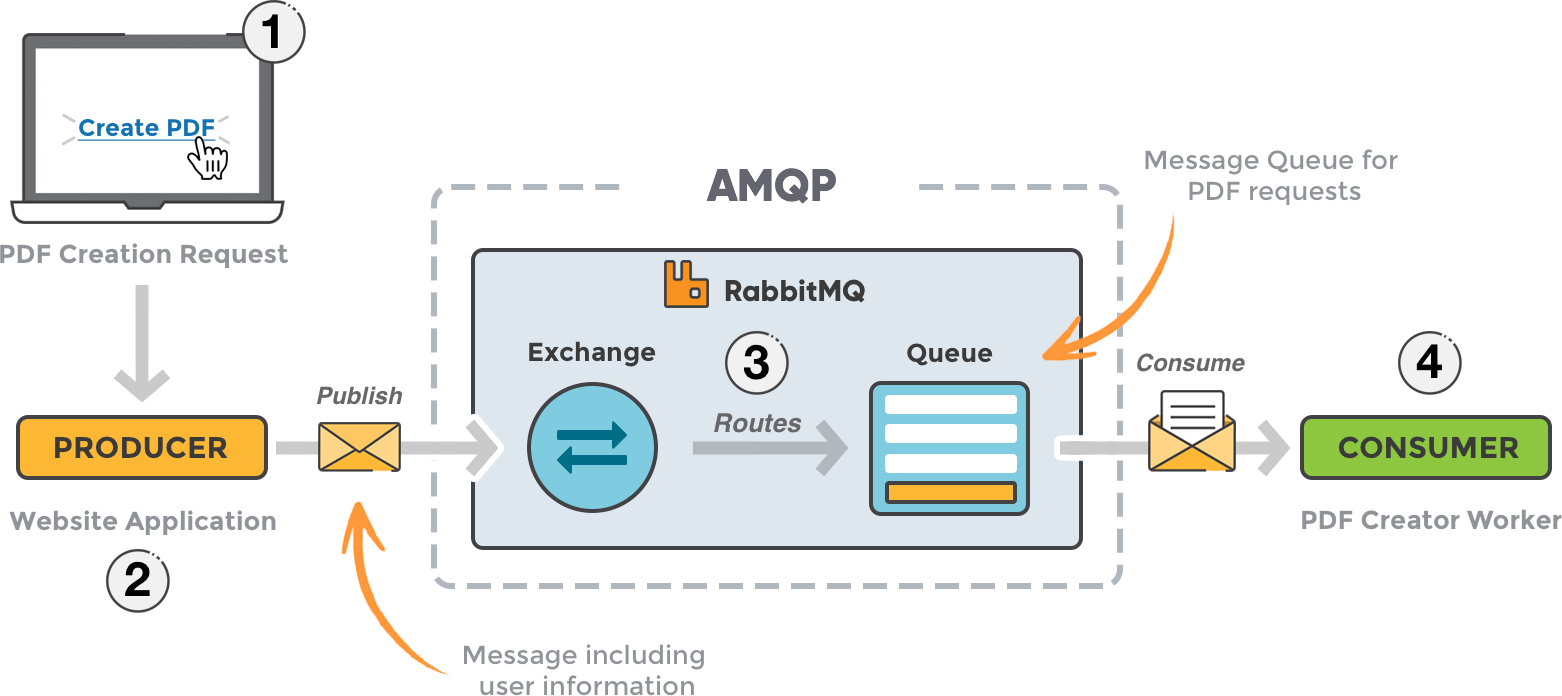
\includegraphics[width=.7\linewidth]{img/rabbitmq.png}
    \end{center}
     %
    \vfill
    %
    \begin{itemize}
        \item[1-2] a producer \alert{publishes} a message towards an \alert{exchange}

        \vfill

        \item[3] the exchange \alert{routes} a \emph{copy} of the message to \emph{a subset of} the queues which are \alert{bound} to the exchange

        \vfill

        \item[3] messages are buffered on the \alert{queues} (hosted by the \alert{broker})

        \vfill

        \item[4] consumers orderly \alert{get} messages from queues
    \end{itemize}

\end{frame}

\begin{frame}{Binding}

    \begin{columns}
        \begin{column}{.5\linewidth}
            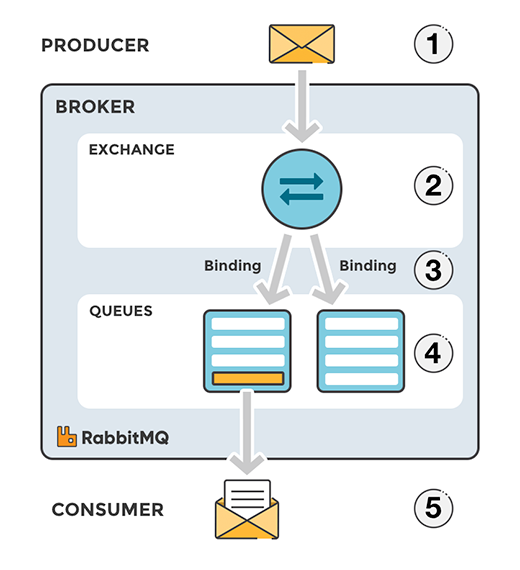
\includegraphics[width=\linewidth]{img/binding.png}
        \end{column}
        \begin{column}{.5\linewidth}
            \begin{itemize}
                \item both exchanges and queues must be \alert{declared by name}\footnotemark
                %
                \begin{itemize}
                    \item i.e. \alert{allocated} on the broker
                \end{itemize}

                \medskip

                \item this implies they'll eventually need to be \alert{disposed}\textsuperscript{\ref{whocan}}

                \medskip

                \item they are \alert{referenced by name}\textsuperscript{\ref{whocan}} during their life span

                \medskip

                \item queue must be \alert{bound}\textsuperscript{\ref{whocan}} to exchanges (step 3)
            \end{itemize}
        \end{column}
    \end{columns}

    \footnotetext{\label{whocan}this can be performed by both producers and consumers}

\end{frame}

\begin{frame}{Exchanges}

    Many sorts of exchanges exist:
    %
    \begin{center}
        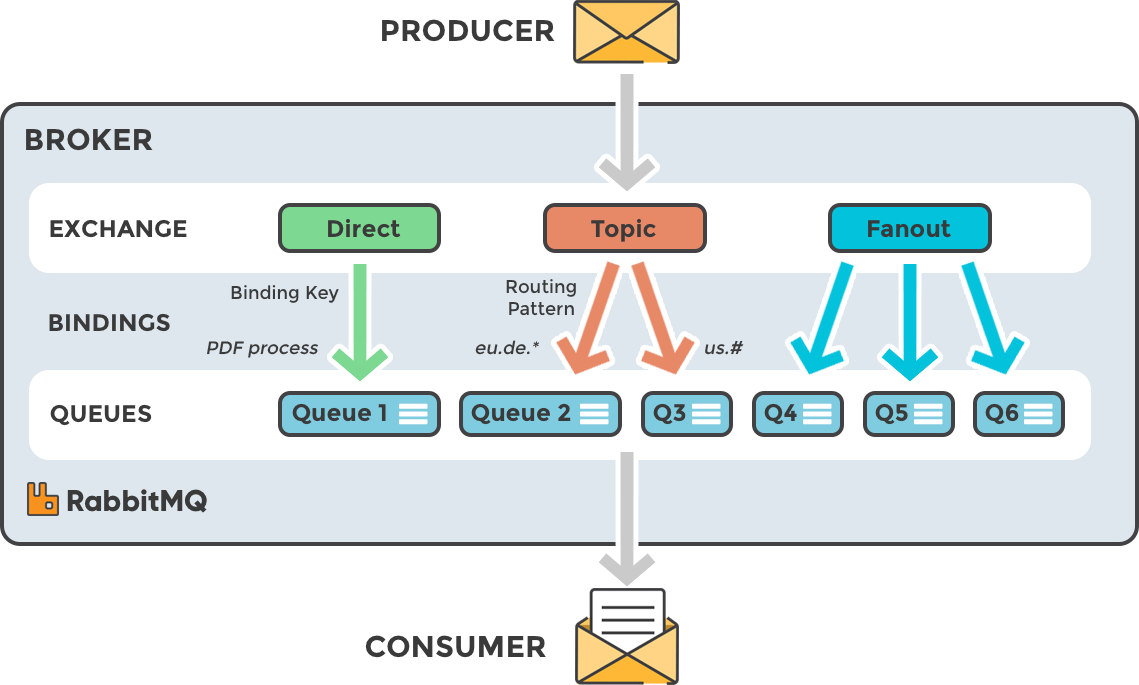
\includegraphics[width=.8\linewidth]{img/exchanges.png}
    \end{center}

\end{frame}

\begin{frame}{Routing with Direct Exchanges}

    \begin{itemize}
        \item Messages are routed to queues in a \alert{round-robin} fashion

        \bigskip

        \item If there's just 1 queue, the routing is \alert{direct}
    \end{itemize}

\end{frame}

\begin{frame}{Routing with Fanout Exchanges}

    \begin{itemize}
        \item Messages are propagated to all bound queues
    \end{itemize}

\end{frame}

\begin{frame}[allowframebreaks]{Routing with Topic Exchanges}

    \begin{center}
        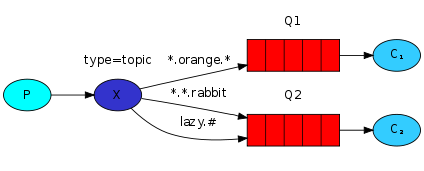
\includegraphics[width=.5\linewidth]{img/routing.png}
    \end{center}

    \bigskip

    \begin{itemize}
        \item Messages are published with a \alert{routing key}

        \medskip

        \item It is then routed to all queues that
        %
        \begin{enumerate}
            \item have been bound to the exchange with a \alert{topic}\ldots
            \item \ldots \alert{matching} the routing key
        \end{enumerate}

        \bigskip

        \item[$\rightarrow$] Queue binding $\approx$ Subscription to topic
    \end{itemize}

    \framebreak

    \begin{block}{Routing keys}\ttfamily\centering
        dot-saparated.sequences.of.words
    \end{block}

    \bigskip

    \begin{block}{Topics}
        \begin{itemize}
            \item dot-separated sequences of words with placeholders:
            %
            \begin{description}
                \item[\texttt{*}] | placeholder for a single word
                \item[\texttt{\#}] | placeholder 0, 1, or more words
            \end{description}
        \end{itemize}
    \end{block}

\end{frame}

\begin{frame}{Queues can be}

    \begin{description}
        \item[server-named] | its name is meaningless for the client, and it is auto-generated by the broker

        \vfill

        \item[exclusive] | can only be used by the entity which declared it, and for as long as its connection to the broker holds

        \vfill

        \item[durable] | the queue is made persistent on the broker-side (i.e., it should survive a broker restart)

        \vfill

        \item[auto-delete] | the queue will be automatically disposed when no longer in use
    \end{description}

\end{frame}

\begin{frame}{Channels vs. Connections}

    \begin{itemize}
        \item producers/consumers must \alert{connect} to the broker

        \vfill

        \item within the scope of a connection, one or more \alert{channels} may be created

        \vfill

        \item via channels producers/consumers can manipulate exchanges and queues

        \vfill

        \item any unexpected action shall close the channel, but not the connection

    \end{itemize}

    \vfill

    \begin{block}{Rule of thumb}
        \begin{itemize}
            \item one connection per producer/consumer
            \item one channel per interaction
        \end{itemize}
    \end{block}

\end{frame}

\section{Exercises}

\begin{frame}
	\frametitle{Overview}

	\begin{block}{Repository}\centering
		\small\url{\labRepo}
	\end{block}

	\vfill

	Activity:
	%
	\vfill
	%
	\begin{enumerate}
		\item Clone the repo onto a \alert{Docker-enabled} host

		\vfill

		\item Start a RabbitMQ service via the provided Docker Compose file:
        %
        \begin{itemize}
            \item[\$] \texttt{docker-compose up}
            %
            \begin{itemize}
                \item launch this command into the directory containing the \texttt{docker-compose.yaml} file
            \end{itemize}
        \end{itemize}

        \vfill

        \item Browse to \url{http://localhost:8080} to use the dashboard
        %
        \begin{itemize}
            \item log in with the credentials from the \texttt{docker-compose.yaml} file
        \end{itemize}

        \vfill

        \item Follow the teacher's explanation and complete the exercises

	\end{enumerate}

\end{frame}

\subsection{Master-Worker}

\startExercise

\begin{frame}{Exercise \currentExercise{} -- Master-Worker}
    \begin{block}{Goal}
        Exploit queues to support a simple master-worker scenario where a master leverages upon an arbitrary amount of workers to count the vowels in its standard input
    \end{block}
\end{frame}

\startExercise

\begin{frame}{Exercise \currentExercise{} -- Instant Messaging}
    \begin{block}{Goal}
        Exploit queues to support a simple command-line instant messaging application for groups of $N \geq 2$ people
        %
        %
        \begin{itemize}
            \item each user is identified by a username
            \item each user should use it terminal to both write and read messages
            \item writing a line on the local standard input should propagate the message to all peers
            \item all received messages should be logged onto the local standard output
            %
            \begin{itemize}
                \item along with the sender's username
            \end{itemize}
        \end{itemize}
    \end{block}
\end{frame}

%===============================================================================
\section*{}
%===============================================================================
\frame{\titlepage}

%===============================================================================
%\section*{\bibname}
%===============================================================================

%\setbeamertemplate{page number in head/foot}{}
%\\\\\\\\\\\\\\\\\\\\\
%\begin{frame}[t,allowframebreaks,noframenumbering]\frametitle{\refname}
%    \tiny
%    \bibliographystyle{plain}
%    \bibliography{sd-lab-queues}
%\end{frame}
%\\\\\\\\\\\\\\\\\\\\\

%%%%%%%%%%%%%%%%%%%%%%%%%%%%%%%%%%%%%%%%%%%%%%%%%%%%%%%%%%%%%%%%%%%%%%%%%%%%%%%
\end{document}
%%%%%%%%%%%%%%%%%%%%%%%%%%%%%%%%%%%%%%%%%%%%%%%%%%%%%%%%%%%%%%%%%%%%%%%%%%%%%%%%

